\chapter{Introduction}

Opposed to Client-server architectures where there are end-hosts and dedicated-hosts (servers),
in P2P Systems there only end-nodes which directly communicate with each other;
they have an ``on/off" behaviour, and they handle \textbf{churn}\footnote{\textit{``churn"} will be a recurring term. In italian it means ``rimescolare'' }.
However, in P2P systems servers are still needed, but only as \textit{bootstrap servers}, typically allowing for new nodes to easily join the P2P network.

Peers' connection in P2P is called \textit{transient}, meaning that connections and disconnections to the network are very frequent.\\
Notice that since each time a peers connects to the P2P network it may have a different IP address, resources cannot be located using IP, but a different method at application layer must be used.

\begin{definition} [P2P System]
   A peer to peer system is a set of autonomous entities (peers) able to auto-organize and sharing a set of distributed resources in a computer network.\\
   The system exploits such resources to give a service in a complete or partial
   decentralized way
\end{definition}

\begin{definition}[P2P System - Alternative definition]
   A P2P system is a distributed system defined by a set on nodes interconnected
   able to auto-organize and to build different topologies with the goal of sharing
   resources like CPU cycles, memory, bandwidth. The system is able to adapt to
   a continous churn of the nodes maintaining connectivity and reasonable
   performances without a centralized entity (like a server)
\end{definition}

\section{Blockchain concepts}
\begin{definition}[Blockchain]
\begin{itemize}
   \item a write-only, decentralized, state machine that is maintained by untrusted
   actors, secured by economic incentive
   \item cannot delete data
   \item cannot be shut down or censored
   \item supports defined operations agreed upon by participants
   \item participants may not know each other (public)
   \item in actors best interest is to play by the rules
\end{itemize}
\end{definition}
\begin{figure}[htbp]
   \centering
   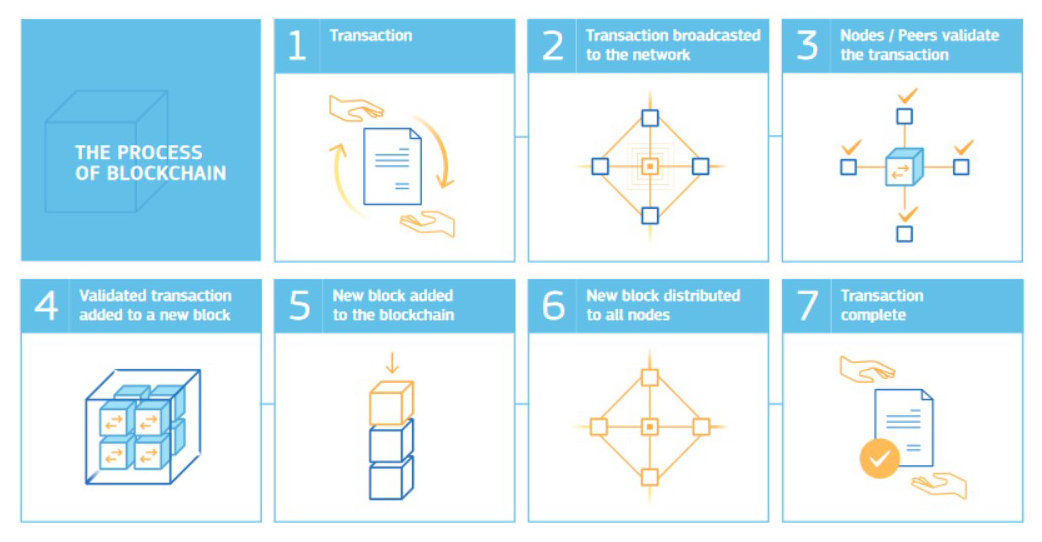
\includegraphics{images/blockchain_process.png}
   \caption{Blockchain process}
   \label{fig:blockchain_process}
\end{figure}

\textit{Bitcoin} were developed as an alternative way to exchange money which wouldn't need intermediaries such as banks.\\
Today, \textit{Ethereum} is becoming more and more popular.\\
\textit{NFT}\footnotemark allow to establish the owner of a digital artwork, by generating a token using a blockchain.

\subsection{TriLemma}
The Blockchain \textbf{trilemma} states that a blockchain \textbf{cannot} simultaneously provide \textit{Decentralization}, \textit{Security} and \textit{Scalability}.

\section{P2P Systems}
\subsection{Semi-Decentralized systems}
An example is \textbf{Napster}, released in 2001.
Napster used servers only to allow users to locate peers which could provide the desired file, delegating the actual file exchange to peers, allowing for a very few server needed.

\note{For the first time users are called \textit{peers}, and the systems implemented in this way \textit{peer-to-peer systems}}

Napster had many strengths common to many P2P systems, from whose emerges the ability of peers to act both as server and a client, but also suffered from weaknesses derived from its centralization, at least for ``node discovery".
Napster centralized server represents a design bottleneck, and also made it target of legal attacks.

\subsection{Fully decentralized systems}
\textbf{Gnutella} is similar to Napster, but here no centralized server exists.
Peers establish \textit{non-transient} direct connections to search files, not to actually transfer them.

\labelitemize{\color{darkred}\textit{Cons}}{\color{darkred}\begin{enumerate}
   \item High network traffic
   \item No structured search
   \item Free-riding
\end{enumerate}}


\section{P2P Overlay network}
In P2P systems there is an overlay network at application level operating on top of the underlying (IP) network.
\begin{figure}[htbp]
   \centering
   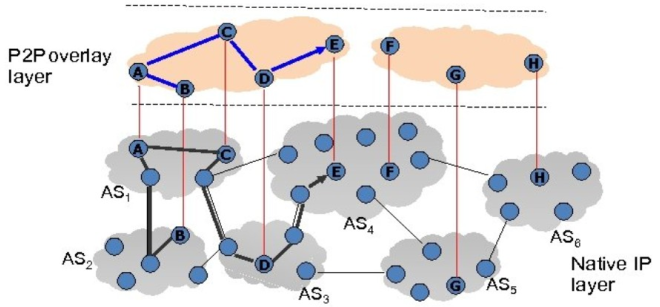
\includegraphics{images/P2Poverlay.png}
   \caption{P2P Overlay networks}
   \label{fig:P2Poverlay}
\end{figure}

A P2P \textbf{protocol} ---defined over the P2P overlay--- defines the set of messages that the peers exchange.

\begin{figure}[htbp]
   \centering
   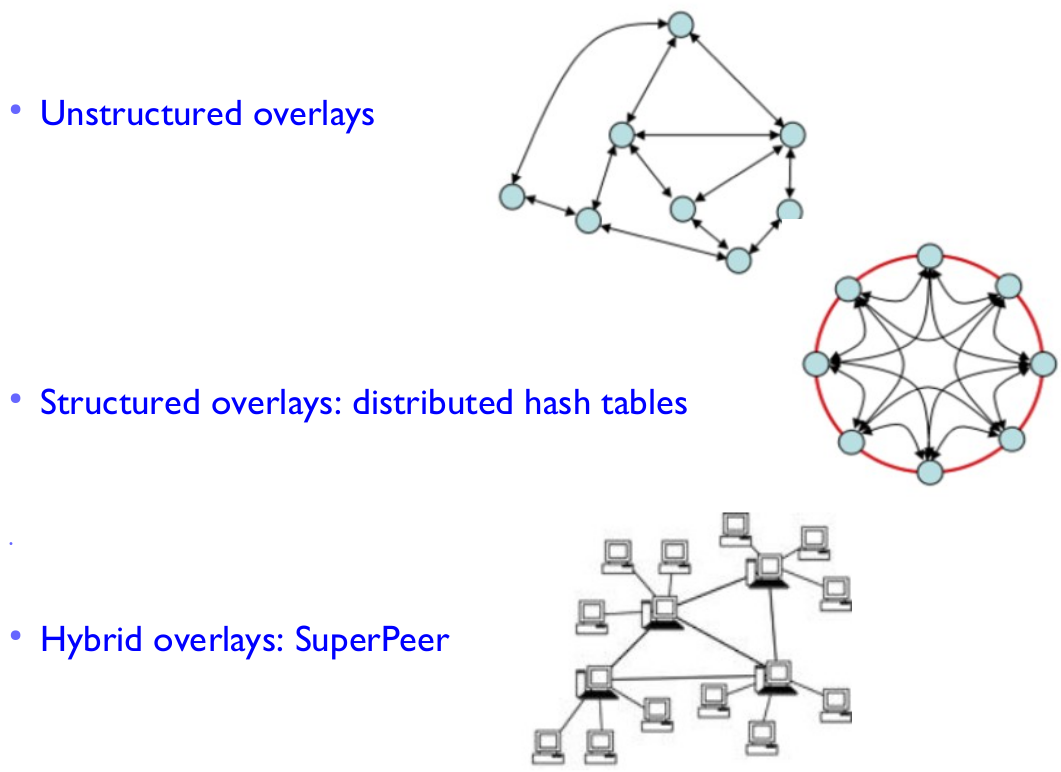
\includegraphics{images/overlayClassification.png}
   \caption{P2P Overlay Network classification}
   \label{fig:overlayClassification}
\end{figure}

\subsection{Unstructured overlay}
\begin{paracol}{2}
   \colfill
   The two key issues here are:
   \begin{itemize}
   \item
   how to \textbf{bootstrap} on the network?
   \item
   how to \textbf{find content} without a central index?
\end{itemize}
\colfill
\switchcolumn
Possible lookup algorithms are the following, but they all are not very scalable, and are costful in terms of performance:
\begin{itemize}
   \item \textbf{Flooding}
   \item \textbf{Expanding ring}
   \item \textbf{Random walk}
\end{itemize}
\end{paracol}
\footnotetext{Non Fungible Tokens}
\note{\texttt{Gnutella}, \texttt{BitTorrent}, \texttt{BitCoin} are examples of unstructured overlay networks.\\
Could not get how bootstrapping works in unstructured overlays.} 

\subsubsectionmark{Test}
\subsubsection{Flooding}
\begin{figure}[htbp]
   \centering
   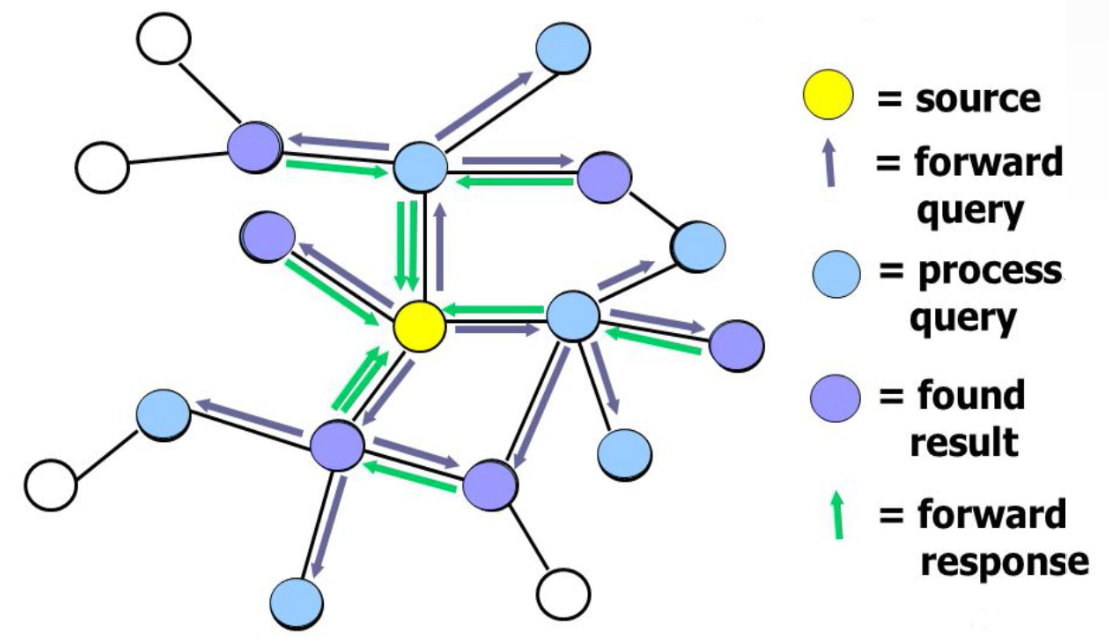
\includegraphics{images/flooding_unstructured.png}
   \caption{Flooding search in unstructured overlay}
   Messages have a \textit{TTL} to limit the number of hops when propagating, but also a \textit{unique identifier} to detect cycles.
   Once the result is found it may be transferred using a direct HTTP connection.

   \note{Flooding is not only for searching, but also to \ul{propagate transactions in the
   P2P network underlying a \textbf{blockchain}}}
   \label{fig:flooding_unstructured}
\end{figure}

\newpage
\subsubsection{Expanding Ring}
\subsubsectionmark{Custom Subsubsection Name}
\begin{figure}[htbp]
   \centering
   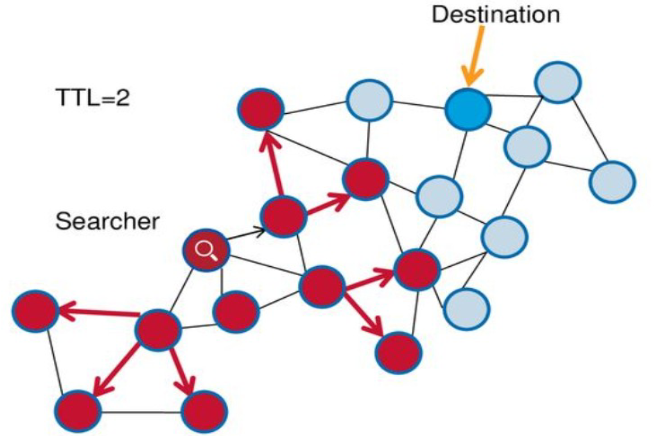
\includegraphics[width=0.45\columnwidth]{images/expandingring2.png}
   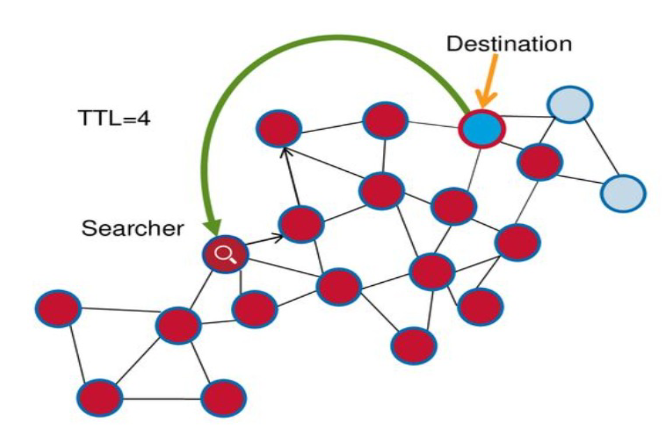
\includegraphics[width=0.45\columnwidth]{images/expandingring4.png}
   \caption{Expanding ring/Iterative Deepening}
   This tecnique consists in repeated flooding towards ---possibly restricted to a subset of randomly selected--- neighbors with an increasing TTL, implementing a BFS search.
   \label{fig:expandingring}
\end{figure}

\subsubsection{Random walk}

\begin{figure}[htbp]
   \centering
   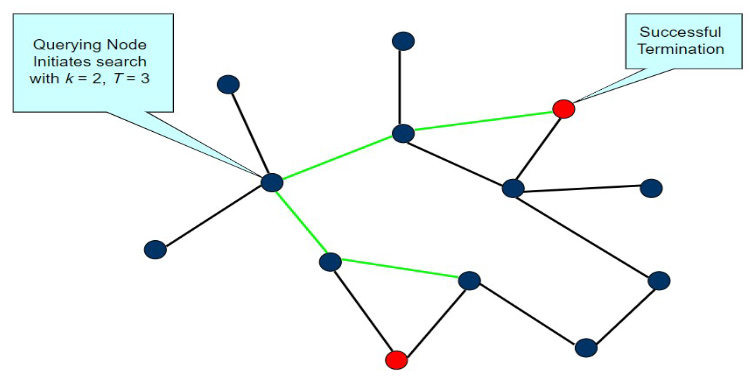
\includegraphics{images/randomwalk.png}
   \caption{Random Walk}
   \label{fig:randomwalk}
   $k$ indicates the number of ``walkers" to be generated by the querying node. Each green path corresponds to a ``walker''.\\
   A path is constructed by taking successive (single) steps in random directions defined by a \textit{Markov Chain}, which is ``memory-less''.
   Note that only one successor node is chosen at each step.\\
   The path is bounded by a TTL.
\end{figure}
Random walk avoids the exponential increase in the amount of messages common in flooding, which becomes an issue for vastly populated networks.\\
Paths can be stopped by a TTL but also by checking periodically with the destination wether the stop condition has been met.\\
A querying node can also bias its walks towards high-degree nodes: higher probability to choose the highest degree neighbor.

\newpage
\subsection{Structured overlays}
\begin{paracol}{2}
   \begin{figure}[htbp]
      \centering
      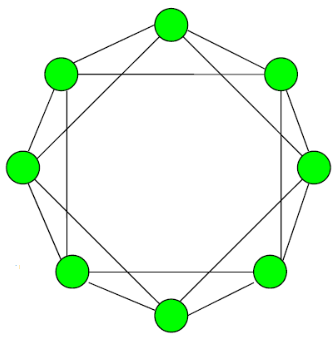
\includegraphics{images/structured_overleay.png}
      \caption{Structured overleay}
      \label{fig:structured_overleay}
   \end{figure}
   \switchcolumn
   The choice of the neighbours is defined according to a given criteria, resulting in a \textbf{structured} overlay network.\\
   The goal is to guarantee scalability by providing:
   \begin{itemize}
      \item \textit{key-based lookup}
      \item  information lookup has a given \textit{complexity} e.g. $\mathcal{O}(log N)$
   \end{itemize}
   
   DHT based solutions, such as \texttt{Chord}, \texttt{Pastry}, \texttt{Kademlia} are examples of structured overlays.
\end{paracol}
   
\subsection{Hierarchical overlays}
\begin{paracol}{2}
   
   \begin{figure}[htbp]
      \centering
      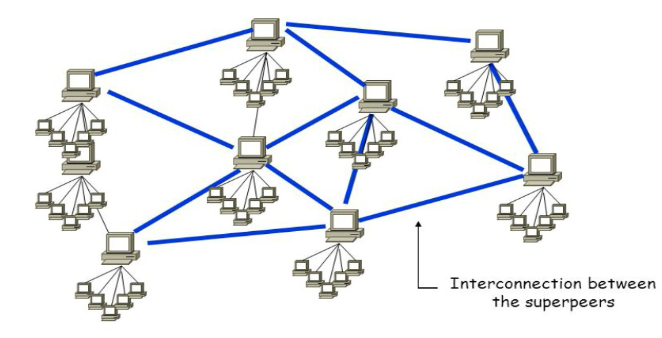
\includegraphics{images/hierarchical_overlay.png}
      \caption{Hierarchical overlay}
   \label{fig:hierarchical_overlay}
\end{figure}

\switchcolumn

Peers connect to \textbf{Super-Peers} which know (\textit{``index''}) Peer resources.
The flooding is restricted to Super-Peers, but still allowing for resources to be directly exchanged between the peers.

Lookup complexity is less and the scalability is improved, but there is a \ul{lower resistance to \textit{super-peers} churn}.

\note{In some cases ---such as Gnutella--- peers are ``\textit{self-promoted}'' to super-peers, while in others they are statically defined.}

\end{paracol}
\subsection{Summary}
\begin{figure}[htbp]
   \centering
   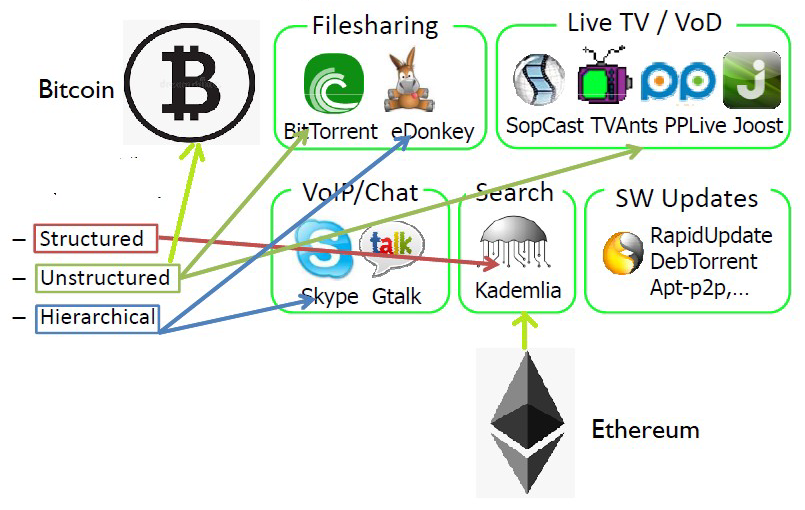
\includegraphics{images/overlays_applications.png}
   \caption{Overlay structure for known applications}
   \label{fig:overlays_applications}
\end{figure}

\begin{figure}[htbp]
   \centering
   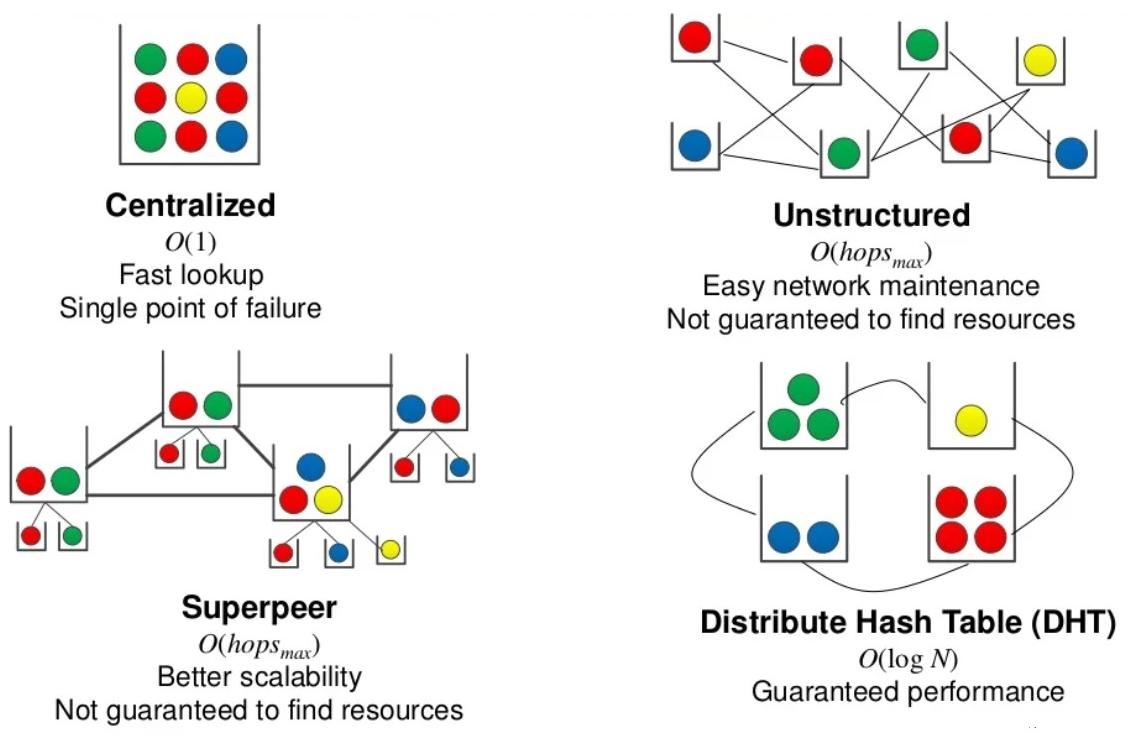
\includegraphics{images/overlays_summary.png}
   \caption{Overlays summary}
   \label{fig:overlays_summary}
   DHT will be discussed in the next chapter
\end{figure}